%% LyX 2.3.6.2 created this file.  For more info, see http://www.lyx.org/.
%% Do not edit unless you really know what you are doing.
\documentclass[english]{scrreprt}
\usepackage[T1]{fontenc}
\usepackage[utf8]{inputenc}
\setcounter{secnumdepth}{3}
\setcounter{tocdepth}{3}
\usepackage{color}
\usepackage{amstext}
\usepackage{graphicx}
\usepackage{esint}

\makeatletter
%%%%%%%%%%%%%%%%%%%%%%%%%%%%%% User specified LaTeX commands.
%\usepackage{epstopdf} % to include .eps graphics files with pdfLaTeX
\usepackage{flafter}   % Don't place floats before their definition
%\usepackage{topcapt}  % Define \topcation for placing captions above tables (not in gwTeX)

\usepackage{xurl}      % better URL setting, uses old url package

\usepackage{xcolor}
\definecolor{darkblue}{rgb}{0,0,0.4}
\usepackage[]{hyperref} % Generates all cross references
\hypersetup{            % Setting options for hyperref package
	breaklinks=true,    % break line with long hyperlinks
	colorlinks=true,    % coloured links
	linkcolor=blue,
	filecolor=magenta,
	urlcolor=darkblue,
	citecolor=blue,
	backref=page
} 

\usepackage{memhfixc}  % remove conflict between the memoir class & hyperref
\usepackage{pdfsync}   % enable tex source and pdf output syncronicity

\usepackage{memhfixc}  % remove conflict between the memoir class & hyperref
\usepackage{pdfsync}   % enable tex source and pdf output syncronicity

\usepackage{alltt}

\makeatother

\usepackage{babel}
\usepackage{listings}
\lstset{language=Python,
extendedchars=false,
frameround=fttt,
numbers=none,
% left line numbers use none,
numberstyle={\tiny},
stepnumber=2,
% line numbers only every so many,
numbersep=9pt,
% how far line numbers from text?,
showspaces=false,
showstringspaces=false,
showtabs=false,
tab={\rightarrowfill},
basicstyle={\small},
keywordstyle={\color{blue}},
commentstyle={\color{green}},
%,
stringstyle={\ttfamily \color{magenta}},
identifierstyle={\color{black}}}
\usepackage[style=authoryear,hyperref=true, backref=true, backrefstyle=three,backreffloats=true,indexing=bib,date=year]{biblatex}
\renewcommand{\lstlistingname}{\inputencoding{latin9}Listing}

\begin{document}
\title{UNESCO-IHE, Delft\\
Transient Groundwater Flow\\
Assignments}
\author{Prof. dr.ir. T.N.Olsthoorn}
\date{\today}

\maketitle
\tableofcontents{}

\renewcommand{\chaptername}{}

\chapter{Assignment Jan 2022. Wells along a river.}

\section{Problem statement}

Consider a region to the right of a straight river which is in direct
contact with a water table aquifer that has a transmissivity of $kD=900\,\mathrm{m^{2}/d}$
or an average saturated thickness of $D=30\,\mathrm{m}$ and a horizontal
conductivity of $k=30\,\mathrm{m/d}$. The specific yield of the aquifer
is $S_{y}=10%\ensuremath{\%}
$.

There is regional groundwater flow directed towards that river at
a rate of $q=0\,\mathrm{m^{2}/d}$.

A groundwater pumping station with one well is installed at $L=1500\,\mathrm{m}$
distance from the river which starts extracting at time $t=0$ at
a rate of $Q=1200\,\mathrm{m^{3}/d}$. For the analysis the aquifer
thickness can be considered constant as given above.

\begin{figure}
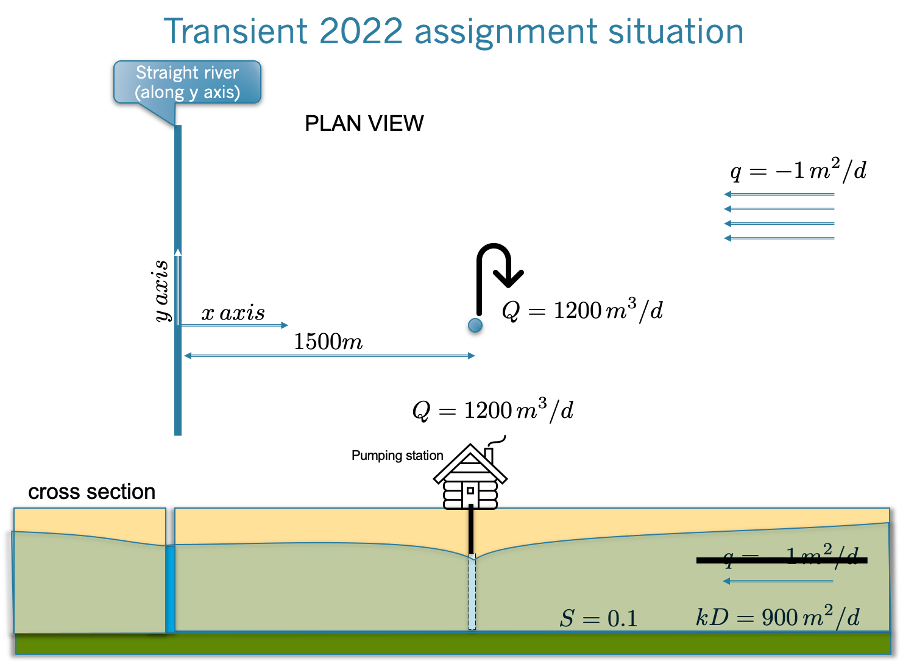
\includegraphics[width=1\textwidth]{pictures/AssJan2022_1}

\caption{Situation, map and cross section.}

\end{figure}

\begin{enumerate}
\item Make a picture of the water table at a line through the pumping well
perpendicular to the river at t the following times 0.001, 1day, 1
week, 1 month, 1 year, 10 years after the start of the extraction.
\item Make a picture of the head contours in top view after 1 month, 1 year
and 10 years.
\item Make a picture of the flow direction in top view after 1 month, 1
year and 10years.
\item Show the inflow from the river
\item The river stage varies like a sine with an amplitude of 2 m and a
cycle time of 1 year. How far from the river can this fluctuation
be felt if one takes 10 cm amplitude as a criterion?
\item Plot the envelopes on top of the steady state (or the head after years
of constant pumping).
\item How much is the delay of the stage wave in the river at the point
where the amplitude is still only 10 cm?
\item There is a sudden shower of rain equal to 240 mm, which raises the
water table suddenly and uniformly. By how much will the water table
rise due to this sudden recharge if it is assumed that all this precipitation
will add to the groundwater?
\item Show the development of the water table over time (for a few times
after the shower took place) by adding its effect to the steady-state
situation (pumping station has been pumping continuously for at least
10 years? 
\end{enumerate}

\section{How to work out the assignment}
\begin{itemize}
\item Work out these questions using Jupyter notebooks in Python. For that
download Anaconda python from the Anaconda website.
\item We’ll introduce this in the course and will practice examples also
in the course.
\item To become familiar google for “Mark Bakker exploratory computing with
Python”. There you’ll find an introduction and a set of notebooks
to exercise as do the 2nd year students at the TUDelft. These tutorials
are really very good.
\item I expect the assignment notebook result two days after the written
exam. The reason is that the mark for the assignment is 30\% and that
of the written exam makes up 70\% of the result, so I need both when
I score the exams.
\end{itemize}

\chapter{Assignment Jan 2021. Wells along a river in a closed valley.}

A groundwater extraction station with three wells is to be realized
in a very long, $L=5\,\mathrm{km}$ wide, almost straight valley.
The valley is bounded by bedrock while the sediments below the water
table can be considered $D=50\,\mathrm{m}$ thick, layer of sand on
top of pratically impervious material. As shown in the cross section
of Figure 1, a river, that may be considered fully penetrating and
in direct contact with the aquifer, flows along one of the valley
walls. The water table is 5 m below ground surface at the center line
of the valley, where the wells are to be installed. As is shown on
the map in Figure 2, the three wells will be placed 500 m apart along
the center line of the valley. Each well will pump $Q=2400\,\mathrm{m^{3}/d}$.

\begin{figure}
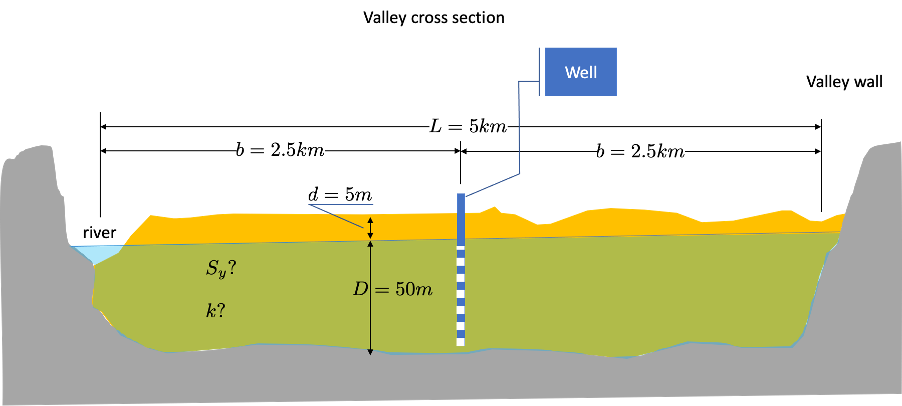
\includegraphics[width=1\textwidth]{pictures/AssJan2021_1}

\caption{Cross section through the valley.}

\end{figure}

One pumping well and three observation wells were installed first,
and a pumping test was done on it to determine the aquifer properties,
i.e. its transmissivity $kD$ and its storage coefficient, i.e. its
specific yield $S_{y}$. The pumping lasted for 1 months (30 days)
at a rate of $Q=600\,\mathrm{m^{3}/d}$. During this time, the heads
in the well and in the piezometers were monitored from which the drawdown
relative to the initial situation was determined. These darwdowns
are provided in a table in an accompanying spreadsheet. The header
of the table shows at which distance from this well the observation
wells were placed. These observation wells (also called piezometers)
are not shown on the cross section and the map because they are too
close to the well to be shown on this scale.

\begin{figure}
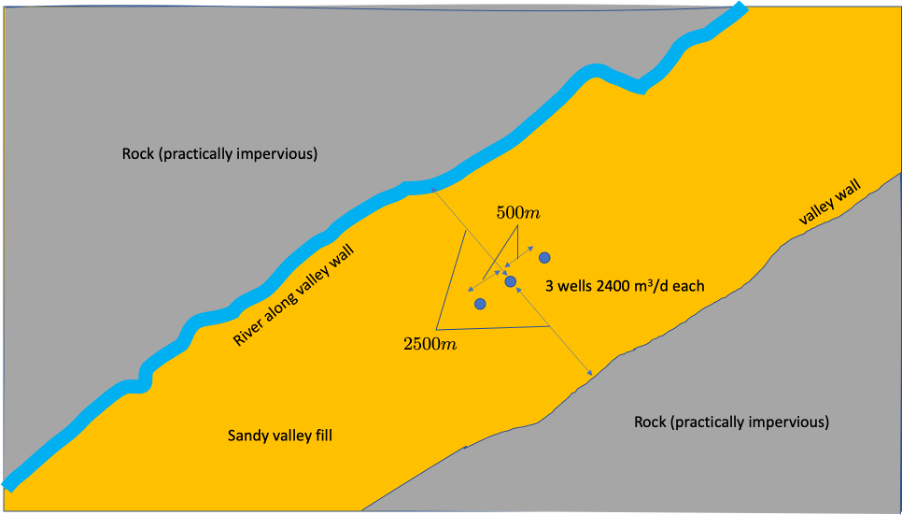
\includegraphics[width=1\textwidth]{pictures/AssJan2021_2}

\caption{Map of the valley with the final three well in place. The observation
wells used in the pumping test are not shown as they are too close
to the well for the scale of this map.}

\end{figure}

Each student obtains a spreadsheet with unique the pumping-test data.
You find the spreadsheet with your name in the folder on BBB named
“Assignment”.

Each student obtains a spreadsheet with unique the pumping-test data.
You find the spreadsheet with your name in the folder on BBB named
“Assignment”. 

\section{Assignment questions}
\begin{enumerate}
\item With the drawdown data given in the accompanying spreadsheet, determine
the aquifer properties kD and Sy.
\item How far out into the aquifer does the drawdown during the pumping
test reach?
\item Is there during the pumping test an influence from the river and or
the valley wall on the drawdowns?
\item What will be the development of the drawdown in the final 3 wells
assuming they are fully penetrating and are not clogged?
\item Show the development of the drawdown along a line perpendicular to
the valley axis through the center well.
\item Show the development of the drawdown along the valley axes through
the 3 wells. 
\item Show the development of the inflow from the river into the aquifer
due to the three wells.
\item Show the drawdown in a map after it has become steady srate.
\item What is the required depth of the pumps, given that the wells have
an extra drawdown due to partial penetration and clogging which doubles
the drawdown relative to the case of unclogged fully penetrating well
and given that the top of the pump has to be at least 1.5 m below
the water table in the well.
\end{enumerate}
Tip: Set the computation up for a single arbitrary point first not
worrying about superposition the results for many points (like along
a line or in a map) and not worrying about superposition across the
river and the valley wall. This can all be included step by step.

\section{The pumping-test data}

TODO: Filled in here.

\chapter{Assignment Jan 2020. Same as Jan 2018}

Essentially the same assignment as in 2018 was used in 2020.

\chapter{Assignment Jan 2019. A building pit next to a river.}

\section{Problem statement}

\begin{figure}
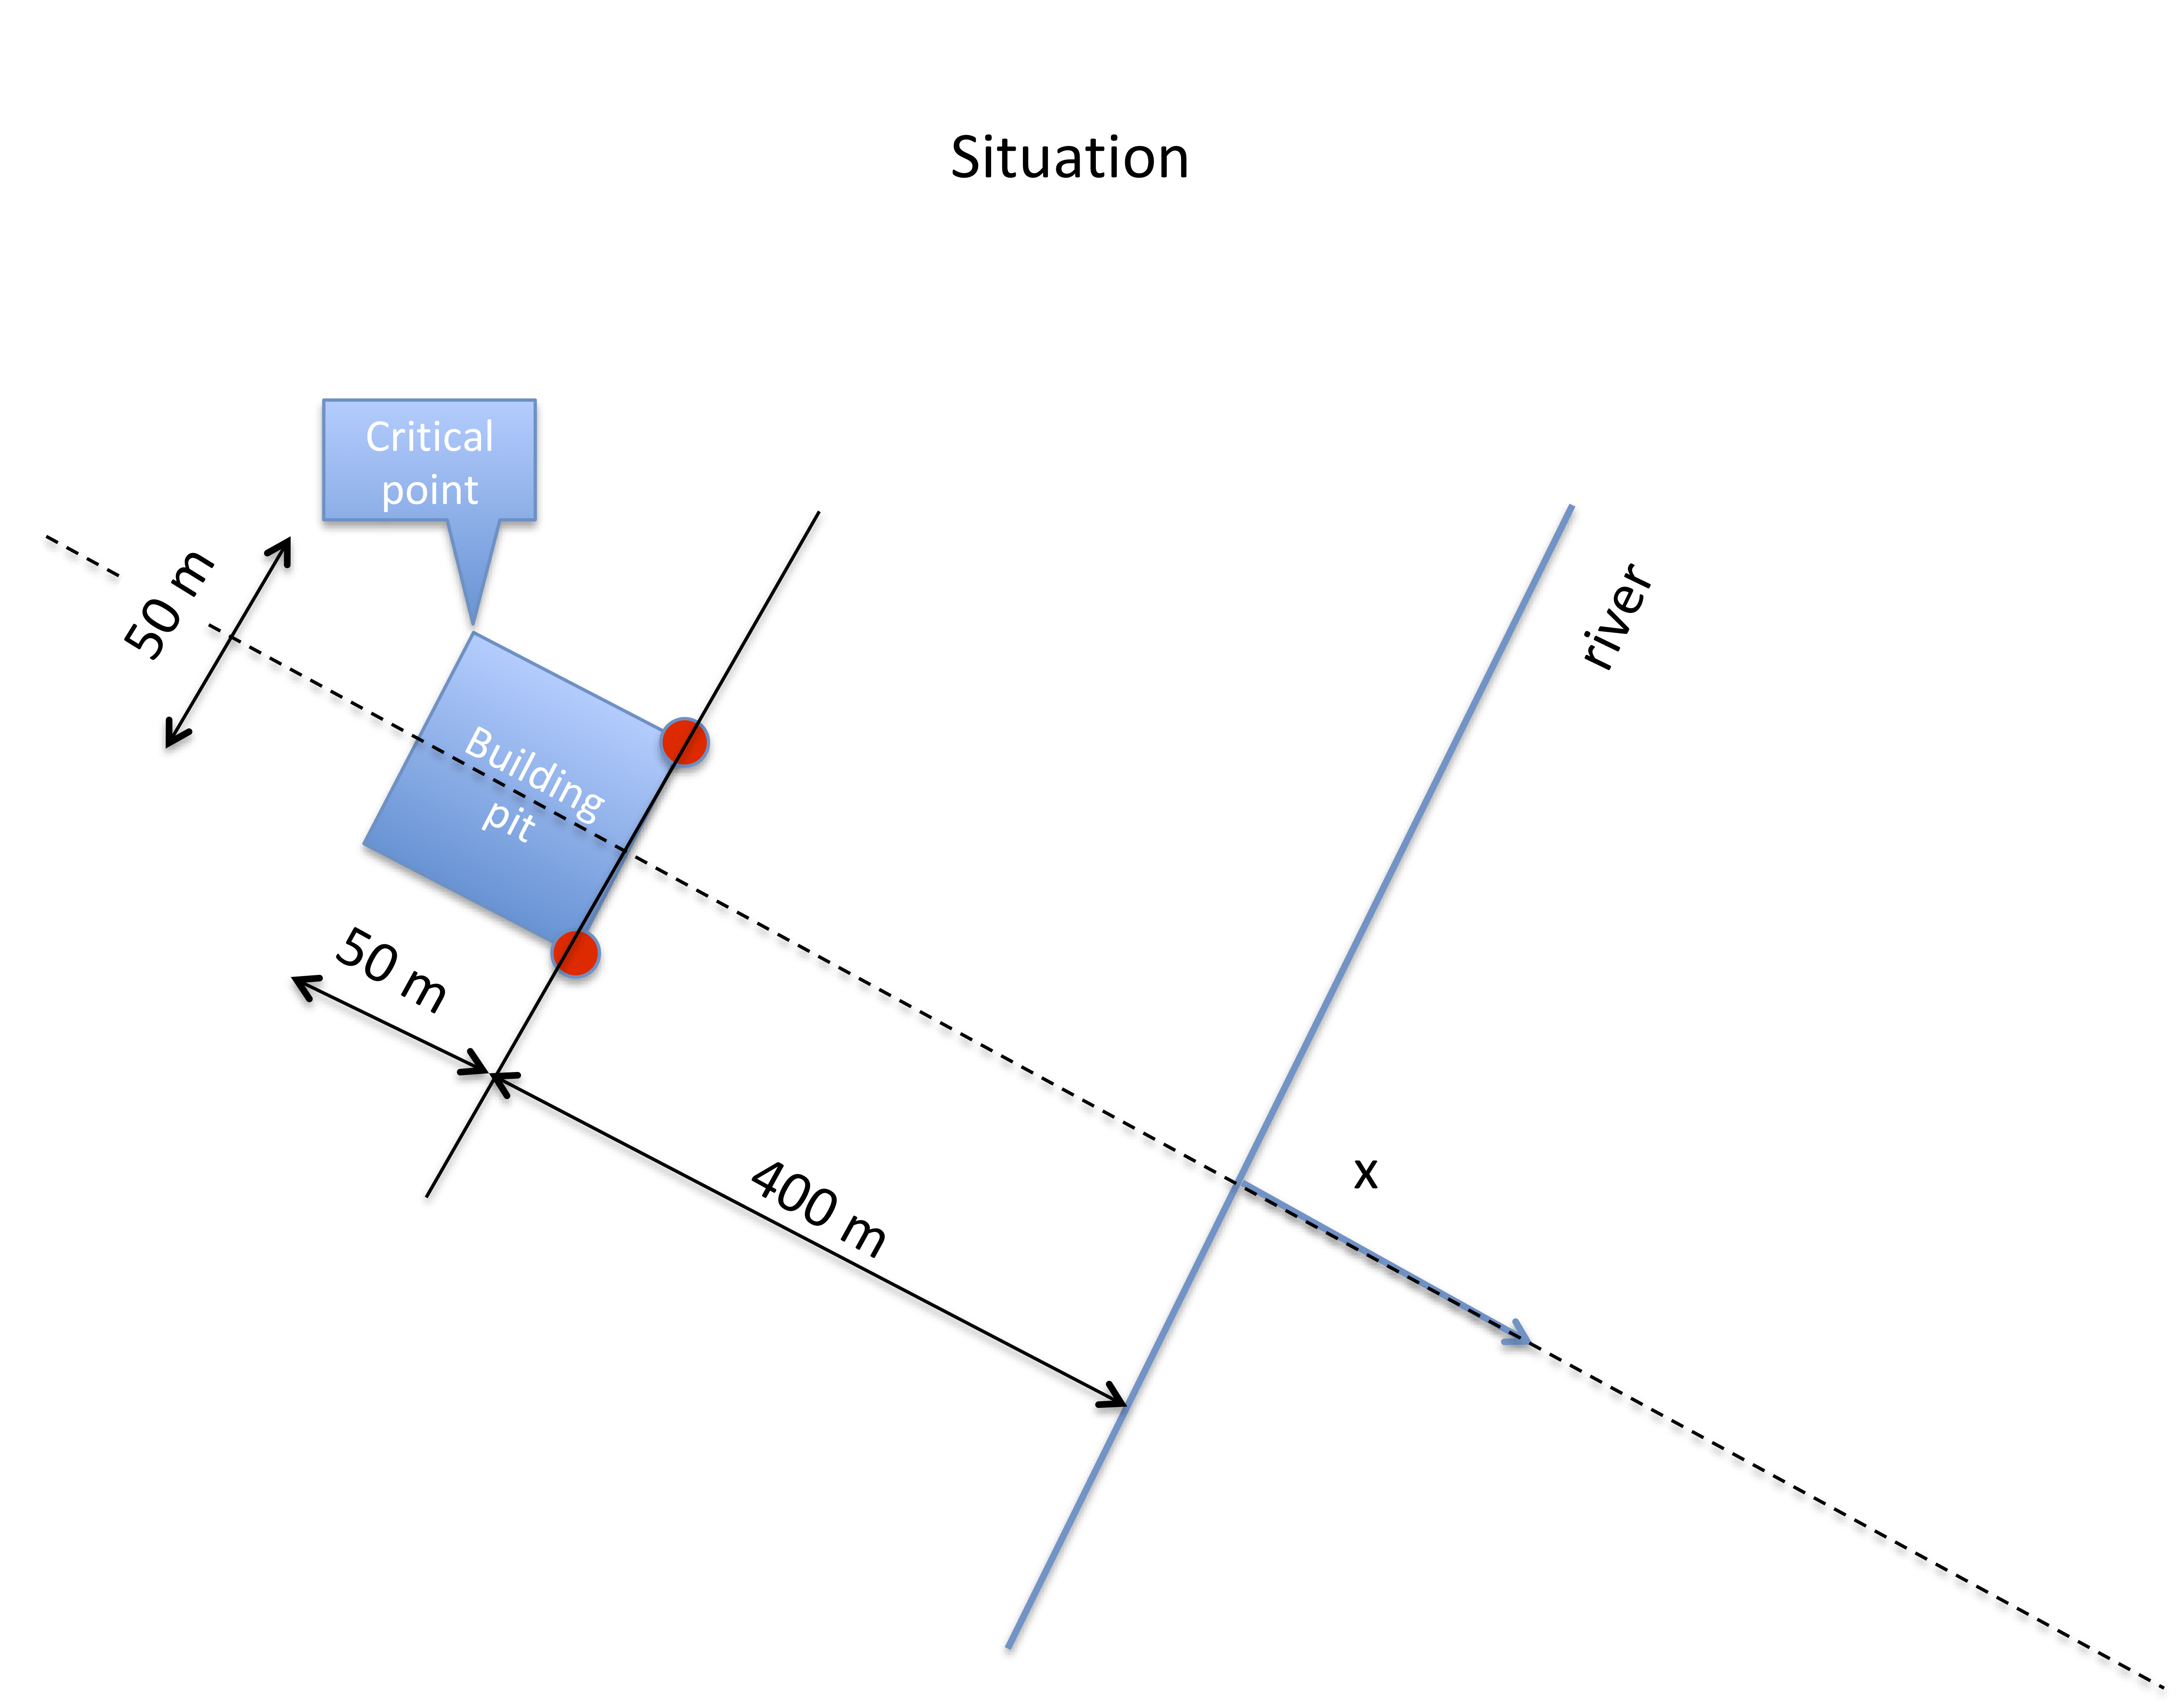
\includegraphics[width=1\textwidth]{pictures/AssJan2019_1}

\caption{Situation sketch.}
\end{figure}

\begin{enumerate}
\item A large construction is to be realized next to a river that is in
direct contact with the aquifer next to it. The building pit measures
50x50 m and river side is at 400 m distance from the river shore.
\item Transmissivity and storage coefficient are given: $kD=900\,\mathrm{m^{2}/d}$,
$S_{y}=0.25$.
\item The drawdown everywhere in the building pit must be at least 5 m,
to be reached within one month of pumping.
\item The pumping will continue after this month for 5 more months during
which the drawdown is to be maintained. However the pumping can be
reduced after the first month. Adjust the pumping once per month,
such that at the end of each month the darwdown fullfils the requied
5 m.
\item After 6 months, pumping is stopped, so that the water levels can restore.
\end{enumerate}

\section{Questions}
\begin{enumerate}
\item On which two corners of the builing pit should you place the two extraction
wells to have most effect?
\item Find the most critical point and make sure that the drawdown is as
required at that point.
\item Show the extraction as a function of time from the start until one
year after the stop. Also plot the drawdown at the critical location
for this period.
\item Compute as a function of time the flow from the river into the groundwater
system. It is assumed that the groundwater head is initially uniform
and equal to the river stage (water level in the river). Do this for
the averate flow during the 6 month of building pit operation (ignore
the variation in the extraction for simplicity).
\item How much time is required after stopping until about 90\% of the drawdown
has disappeared?
\item After exactly 3 months, the water level in the river rises suddenly
by 1 m and stays so during one month, after which it suddenly returns
to its original level.
\item To what extent does this wave affect the water level in the building
pit if no measure is taken?
\item What must be the extraction during this month to guarantee that the
building pit fulfills the required 5 m drawdown relative to the original
water level? If both effects do not overlap, say so, and explain what
you could to as building-pit owner to better counteract the effect
of the wave in the river stage on the head below the building pit
\item If the river is influenced by sea tide, such that its level fluctuates
twice a day between +1 and -1 m relative to the average value. How
does this tide influence the required pumping? Is the location of
the most critical point still the same?
\item How much is the delay between the tide in the river and the fluctuation
at the critical point in the building pit?
\end{enumerate}

\section{Hints}
\begin{enumerate}
\item Work out the assigment in this Jupyter notebook. Take some time to
become familiar with it. There is a tremendous amount of help on the
internet to get you going. The site on `github.com/Olsthoorn/TransientGroundwaterFlow`
hold numerous examples from the syllabus in the form of `jupyter notebooks`.
\item Also refer to the notebooks for the second year students of the TUDelft
by Mark bakker (search for `Bakker exploratory` computing to find
them).
\item You will gain some experience with the Notebooks (see their help)
\begin{enumerate}
\item with python
\item with numpy
\item with functions in scipy
\end{enumerate}
\item Make sure your assigment is a self-contained document, that you could
also export as html or pdf for sharing to those who do not have python
installed.
\end{enumerate}

\chapter{Assignment Jan 2018. Water company uses ASR system to prevent river
inflow during summer.}

The assignment is essentially the same as the one of 2017.

\chapter{Assignment Jan 2017. Water company uses ASR system to prevent extraction
from tiver during summer}

\section{Problem statement}

A water company extracts water from a small river to treat and distribute
it as drinking water for the population of a small town nearby. This
is not a problem in winter. However, due to growing demand for drinking
water and growing environmental concern, extraction has become more
and more problematic during summers when the discharge of this small
river is at its lowest. The environmental agency has recently even
forbidden to further extract water from the river during the summer
months.

\begin{figure}
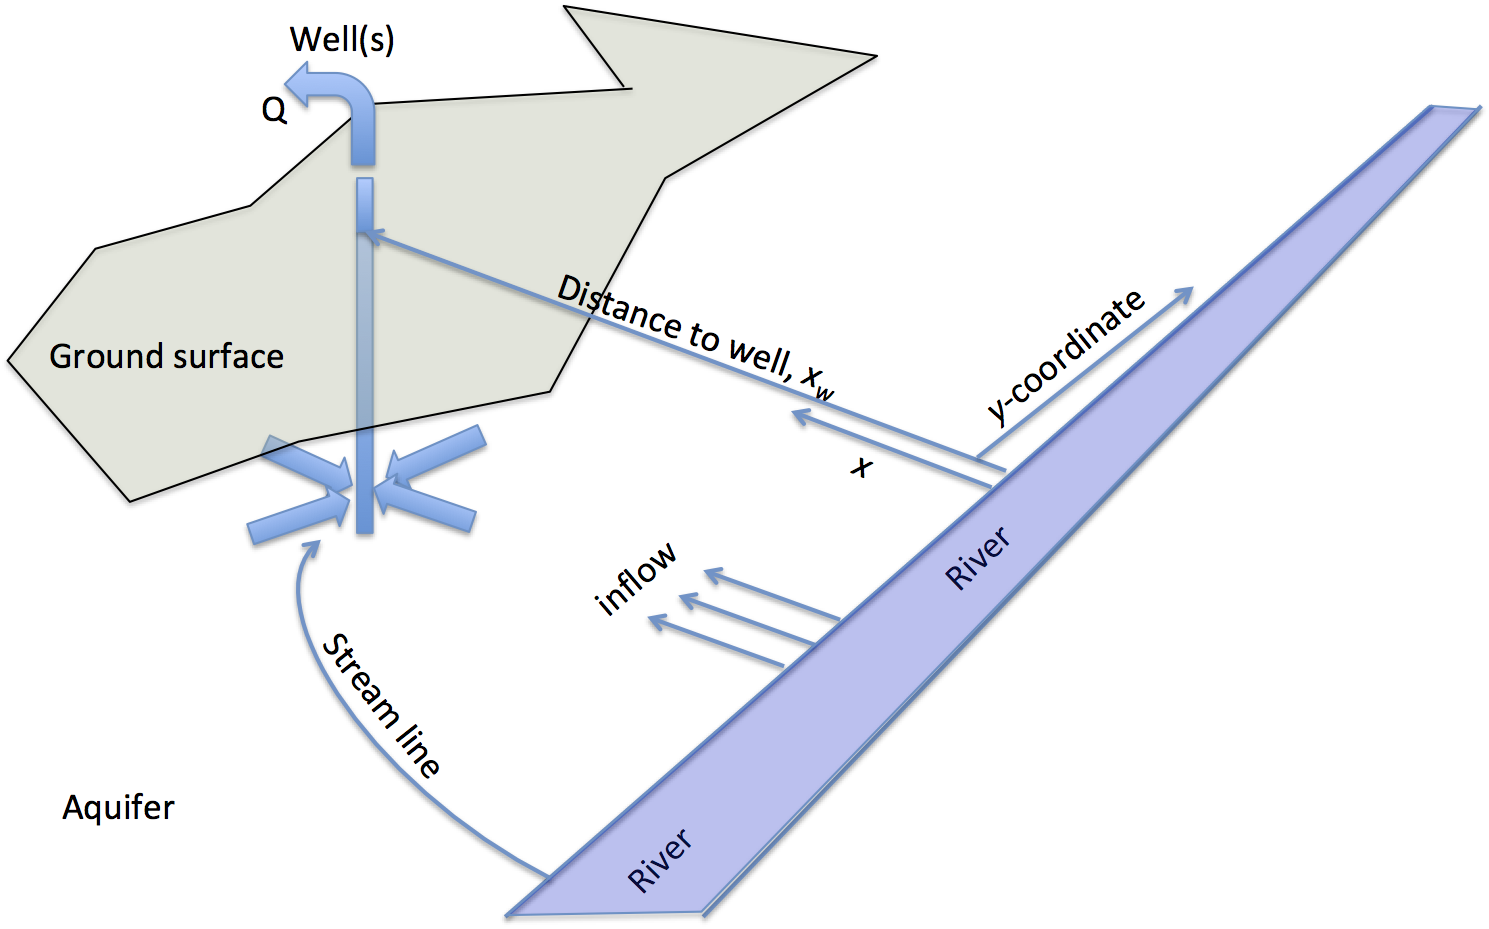
\includegraphics[width=1\textwidth]{pictures/AssJan2018_1}

\caption{Situation sketch.}
\end{figure}

In order to solve the problem that this causes for the drinking water
supply, the drinking water company has suggested an \textquotedbl Aquifer
Storage and Recovery\textquotedbl{} system (these so-called ASR systems
are becoming more and more popular). It wants to take in more river
water during winter and inject it through a well (or wells) at some
distance from the river into the local water-table aquifer, so that
this water can be extracted during the next summer. This way, no water-intake
will be necessary during the summer months.

However, the debate that took off between the water company and the
environmental agency focuses on whether, or to what extent, this ASR
system really makes sense. Can you really store the water in winter
and extract it during summer without substantially affecting the already
low summer-discharge of the river? Will not much of the stored water
flow back to the river through the aquifer during winter? And would
the extraction not induce an infiltration from the river into the
aquifer during summer, so that there is still a water intake, the
only differece now being that it will be invisible?

It's your task as hydrologist of the environmental agency to answer
this question and illustrate it quantitatively and also explain it
clearly. Your explanation should include why and how you derived your
answer. It should show the math and the code.

It is obvious that ASR will work if the distance between the well
and the river is large enough. But how large is large enough, and
on what does it depend? The water company suggested a distance of
500 m from the river. Should the environmental agency agree?

\section{Hints and further information:}
\begin{enumerate}
\item To analyse this system, at least coarsely, simplify the injection
and extraction regime and apply superposition. Superposition allows
to only consider the well and treat the river as a fixed-head boundary
using a mirror well. Simplify the river to a straight line along the
y-axis and place the well at distance $x_{w}$ from this line at coordinate
$(x_{w},0)$. That is, the x-axis is perpendicular to the river.
\item The drinking water demand, $Q$, is considered constant year-round
at $150\,\mathrm{L/d}$ per inhabitant for the 10000 inhabitants of
the town.
\item Assume the following injection and recovery regime:
\begin{enumerate}
\item The water company well extracts during 3 summer months (June, July,
Aug) its full demand
\item It compensates that during 6 winter months (October-March) by injecting
half its daily capacity.
\item There is neither injection nor extraction during the months April,
May and September.
\end{enumerate}
\item The idea is to analyse this ASR system by computing the exchange between
the aquifer and the river due to the well.
\item When you have coded the problem for this particular distance of 500
m, experiment with this distance to come up with a distance that realy
makes sense in terms of not inducing loss of river water during the
summer months. That is, try 1000 and 2000 m.
\item Use $kD=900\,\mathrm{m^{2}/d}$, $S_{y}=0.2$.
\end{enumerate}

\section{Steps to take:}
\begin{enumerate}
\item Use Theis' well function to compute drawdowns:
\[
s(t,t)=\frac{Q}{4\pi kD}\mathrm{W}(u)\mbox{, with }\mathrm{W}(u)=-scipy.special.expi(-u)\mbox{ and }u=\frac{r^{2}S}{4kDt}
\]
\item From Theis' well function\\
\[
\mathrm{W}(u)=\intop_{u}^{\infty}\frac{e^{-y}}{y}dy
\]
derive the flow $Q(r,t)\,\mathrm{[L^{3}/T]}$ and the specific discharge
$q(r,t)\,\mathrm{[L^{2}/T]}$ in the aquifer at distance $r$ from
the well.
\item To simulate the river, apply a mirror well.
\item Compute the exchange between aquifer and river, derive the specific
discharge $q\,\mathrm{[L^{2}/T]}$ perpendicular to the river at an
arbitrary point $y$.
\item Compute this specific discharge for a large number of points between
$-ax_{w}<y<ax_{w}$, where $a$ is sufficiently large, thus covering
a large enough track of the river to capture about the full induced
exchange between aquifer and the river. See below how appropriate
$y$-coordinates can be generated in Python.
\item Numerically integrate this specific discharge along the river to obtain
the total exchange between river and aquifer. (Numerical integration
is easy when uing the Simpson's trampezium rule).
\item Having the code to do this for a single time, it can readily be extended
for a large number of times.
\item Check that for large times, the total flow between aquifer and river
should be about the total discharge of the well if the well is continuously
injecting.
\item Finally simulate the actual flow regime with 6 month injection and
3 months extraction as explained above. Simulate for a period of 5
years. This simulation requires superposition in time.
\end{enumerate}
Appropriate $y$-coordinates may be generated in Python as follows:

\inputencoding{latin9}\begin{lstlisting}
y = np.hstack(( -np.logspace(0, np.log10(a * xw), Np)[::-1], np.logspace(0, np.log10(a * xw), Np))
\end{lstlisting}
\inputencoding{utf8}
Where $a$ may be taken 10 and the number of points, $N_{p}$, can
be taken 500 for example.

\section{Suggestions}
\begin{enumerate}
\item 1. It is probably easiest to analyze everything in time units of months
instead of days, 5 years time then runs from 0 to 60 months.
\item 1. Learn to define and use functions in Python to keep overview and
prevent repeating code.
\item 2. If you consider this too complicated, then anlyse at least the
situation for only the river point closest to the well.
\item 3. Start by plotting the head.
\item 4. When this works focus on the discharge.
\item 1. Don't hesitate to ask questions and for help.
\end{enumerate}

\section{The data as a csv (comma separated values)}

You can select the values below and copy-paste them in a text file
to be read by python (use the pandas module for convenience for working
with tables and reading them including excel sheets and csv files.)

\inputencoding{latin9}\begin{lstlisting}
date,n,month,year,Qfac,Q,dQ,tch
2010-01-01,1,1,2010,0.5,750,750,0
2010-02-01,2,2,2010,0.5,750,0,31
2010-03-01,3,3,2010,0.5,750,0,59
2010-04-01,4,4,2010,0,0,-750,90
2010-05-01,5,5,2010,0,0,0,120
2010-06-01,6,6,2010,-1,-1500,-1500,151
2010-07-01,7,7,2010,-1,-1500,0,181
2010-08-01,8,8,2010,-1,-1500,0,212
2010-09-01,9,9,2010,0,0,1500,243
2010-10-01,10,10,2010,0.5,750,750,273
2010-11-01,11,11,2010,0.5,750,0,304
2010-12-01,12,12,2010,0.5,750,0,334
2011-01-01,13,1,2011,0.5,750,0,365
2011-02-01,14,2,2011,0.5,750,0,396
2011-03-01,15,3,2011,0.5,750,0,424
2011-04-01,16,4,2011,0,0,-750,455
2011-05-01,17,5,2011,0,0,0,485
2011-06-01,18,6,2011,-1,-1500,-1500,516
2011-07-01,19,7,2011,-1,-1500,0,546
2011-08-01,20,8,2011,-1,-1500,0,577
2011-09-01,21,9,2011,0,0,1500,608
2011-10-01,22,10,2011,0.5,750,750,638
2011-11-01,23,11,2011,0.5,750,0,669
2011-12-01,24,12,2011,0.5,750,0,699
2012-01-01,25,1,2012,0.5,750,0,730
2012-02-01,26,2,2012,0.5,750,0,761
2012-03-01,27,3,2012,0.5,750,0,790
2012-04-01,28,4,2012,0,0,-750,821
2012-05-01,29,5,2012,0,0,0,851
2012-06-01,30,6,2012,-1,-1500,-1500,882
2012-07-01,31,7,2012,-1,-1500,0,912
2012-08-01,32,8,2012,-1,-1500,0,943
2012-09-01,33,9,2012,0,0,1500,974
2012-10-01,34,10,2012,0.5,750,750,1004
2012-11-01,35,11,2012,0.5,750,0,1035
2012-12-01,36,12,2012,0.5,750,0,1065
2013-01-01,37,1,2013,0.5,750,0,1096
2013-02-01,38,2,2013,0.5,750,0,1127
2013-03-01,39,3,2013,0.5,750,0,1155
2013-04-01,40,4,2013,0,0,-750,1186
2013-05-01,41,5,2013,0,0,0,1216
2013-06-01,42,6,2013,-1,-1500,-1500,1247
2013-07-01,43,7,2013,-1,-1500,0,1277
2013-08-01,44,8,2013,-1,-1500,0,1308
2013-09-01,45,9,2013,0,0,1500,1339
2013-10-01,46,10,2013,0.5,750,750,1369
2013-11-01,47,11,2013,0.5,750,0,1400
2013-12-01,48,12,2013,0.5,750,0,1430
2014-01-01,49,1,2014,0.5,750,0,1461
2014-02-01,50,2,2014,0.5,750,0,1492
2014-03-01,51,3,2014,0.5,750,0,1520
2014-04-01,52,4,2014,0,0,-750,1551
2014-05-01,53,5,2014,0,0,0,1581
2014-06-01,54,6,2014,-1,-1500,-1500,1612
2014-07-01,55,7,2014,-1,-1500,0,1642
2014-08-01,56,8,2014,-1,-1500,0,1673
2014-09-01,57,9,2014,0,0,1500,1704
2014-10-01,58,10,2014,0.5,750,750,1734
2014-11-01,59,11,2014,0.5,750,0,1765
2014-12-01,60,12,2014,0.5,750,0,1795
2015-01-01,61,1,2015,0.5,750,0,1826
2015-02-01,62,2,2015,0.5,750,0,1857
2015-03-01,63,3,2015,0.5,750,0,1885
2015-04-01,64,4,2015,0,0,-750,1916
2015-05-01,65,5,2015,0,0,0,1946
2015-06-01,66,6,2015,-1,-1500,-1500,1977
2015-07-01,67,7,2015,-1,-1500,0,2007
2015-08-01,68,8,2015,-1,-1500,0,2038
2015-09-01,69,9,2015,0,0,1500,2069
2015-10-01,70,10,2015,0.5,750,750,2099
2015-11-01,71,11,2015,0.5,750,0,2130
2015-12-01,72,12,2015,0.5,750,0,2160
2016-01-01,73,1,2016,0.5,750,0,2191
2016-02-01,74,2,2016,0.5,750,0,2222
2016-03-01,75,3,2016,0.5,750,0,2251
2016-04-01,76,4,2016,0,0,-750,2282
2016-05-01,77,5,2016,0,0,0,2312
2016-06-01,78,6,2016,-1,-1500,-1500,2343
2016-07-01,79,7,2016,-1,-1500,0,2373
2016-08-01,80,8,2016,-1,-1500,0,2404
2016-09-01,81,9,2016,0,0,1500,2435
2016-10-01,82,10,2016,0.5,750,750,2465
2016-11-01,83,11,2016,0.5,750,0,2496
2016-12-01,84,12,2016,0.5,750,0,2526
2017-01-01,85,1,2017,0,0,-750,2557
2017-02-01,86,2,2017,0,0,0,2588
\end{lstlisting}
\inputencoding{utf8}

\chapter{Assignment Jan 2016. Several exercises based on the syllabus.}

This is the last assignment using Excel. Later ones all used Python
(Jupyter notebooks), which are much more powerfull for this kind of
work and also freely available, where Excel is not. The workout in
Excel is availale. Here we will use Python.

\section{Setup}

Assignments are to be done in Excel, but those who want, can do them
in Python; we’ll stick to Excel in class.

I want you to explain why you took this and that step. The essence
is that you show that you understand what is at stake; the exact numerical
answer is less important. Clearly, everybody should workout his/her
own assignment. The assignment is split into 7 parts. Each can be
done on a single worksheet, hence all can be joined in a single Jupyter
notebook.

\section{Capillary rise}

For grain sizes $d=0.002\mbox{, }0.02\mbox{, }0.2\mbox{ and }2\,\mathrm{mm}$
determine the capillary rise. Assume the angle between the free surface
and the straw wall in the equivalent straw is $20^{o}$ and the surface
tension is $\tau=75\times10^{-3}\,\mathrm{N/m}$. Also assume that
the pore diameter, $r$, is 20\% of the grain diameter $d$. The density
of Water $\rho_{w}=1000\,\mathrm{kg/m^{3}}$ and gravity $g=10\,\mathrm{m/s^{2}}$which
is the same as $\text{10\,N/kg}$

\section{Tidal fluctuations}

Let the solution to the diffusion equation for the confined aquifer
be

\[
s(x,t)=A\exp(-ax)\sin(\omega t-ax)
\]

and let $kD=1000\,\mathrm{m^{2}/d}$, $S=10^{-2}$ and the amplitude
$A=2\,\mathrm{m}$.
\begin{enumerate}
\item Take time in days and show graphically the head change $s(x,t)=\phi(x,t)-\phi_{0}$
as a function of $x$ for some values of $t$, assuming the constant
$\theta_{0}=\pi/3$. Use times $t=2/24\mbox{, }4/24\mbox{, }6/24\mbox{ and }8/24\,\mathrm{days}$
\item Add the graph of the envelope of the wave as a function of $x$.
\item Also make a graph of the discharge $Q(x,t)$ showing $Q$ as a function
of $x$ for the same times.
\item How far inland can we measure the effect of the tide if our water
level logger device registers any head change beyond 1 cm ?
\item What is the velocity of the wave?
\item What is delay of the wave is at $x=1000\,\mathrm{m}$ from the shore
(or show the delay
\item graphically as function of $x$)
\item What the wavelength? Verify this in you graph.
\item Add the envelopes for the case that the storage coefficient is $S=10^{-2}$
instead of $S_{y}=0.2$.
\item What is the distance over which the envelope reduces by a factor 2?
\end{enumerate}

\section{Temperature variation in the subsurface:}

Consider a sinusoidal fluctuation of the temperature at ground surface.
Assume the soil to be saturated with porosity $\epsilon=0.35$, while
the heat capacity of grains of the aquifer is $\rho_{g}c_{g}=2650\times800\,\mathrm{J/m^{3}/K}$
and the heat capacity of the water is $\rho_{w}c_{w}=1000\times4200\,\mathrm{J/m^{3}/K}$.
Notice that K stands for the absolute temperature, Kelvin, which is
the same as $\mathrm{Celsius}+273.1\,\mathrm{K}$.

Assume that the average year-round ground temperature is $10^{o}\mathrm{C}$
and the fluctuation is $\pm8^{o}\mathrm{C}$. Also use $\lambda_{w}=2\,\mathrm{W/K/m}$
and $\lambda_{g}=4\,\mathrm{W/K/m}$.

Show the temperature envelopes for
\begin{itemize}
\item Diurnal (=daily)
\item Seasonal (=yearly)
\item Centennial (=one wave lasting a century)
\end{itemize}

\section{Effect of a sudden change of the water level in a river}

An aquifer with transmissivity $kD=400\,\mathrm{m^{2}/d}$ and storage
coefficient $S_{y}=0.1$ is in direct contact with a river. The water
level in the river suddenly changes by $A=2\,\mathrm{m}$.
\begin{enumerate}
\item 1. Show the effect of this change as a function of time for points
at $x=10\mbox{, }100\mbox{ and }1000\,\mathrm{m}$ from the river.
\item 2. How long does it take until the head change s in these three points
equals 10 cm?
\item 3. Show the discharge over time at these points.
\end{enumerate}

\section{Decay of head in a strip of land of given width (characteristic time
of the groundwater system)}

Consider a cross section of an aquifer with transmissivity $kD=200\,\mathrm{m^{2}/d}$
and $S=0.1$ between 2

straight canals at a distance $L=500\,\mathrm{m}$ from each other.
The cross-section runs from $x=-L/2$ to $x=+L/2$.
\begin{enumerate}
\item Implement the head caused by a sudden rise of water level by 2 m at
both sides of the strip using superposition of a sufficient number
of “mirror” strips of land.
\item Show that this is essentially the same as the formula we implemented
in class:\\
\[
s\left(x,t\right)=A\frac{4}{\pi}\sum_{i=1}^{\infty}\left(\frac{\left(-1\right)^{i-1}}{2i-1}\cos\left[\left(2i-1\right)\pi\frac{x}{L}\right]\exp\left[-\left(2i-1\right)^{2}\pi^{2}\frac{kD}{L^{2}S}t\right]\right)
\]
\item Show the situation on 1 to 8 halftimes.
\end{enumerate}

\section{Implement the Theis and Hantush well functions $\mathrm{W}(u)$ and
$\mathrm{W}(u,r/\lambda)$ as a function of $1/u$}
\begin{enumerate}
\item Compute and show the type curves using the implementation of the Theis
and Hantush well functions. Show the type curves of the Theis and
Hantush function versus $1/u$. Use a data range for $10^{-3}<u<10^{2}$.
\item Consider a confined aquifer with transmissivity $kD=1000\,\mathrm{m^{2}/d}$
and storage coefficient $S=0.001$. Let there be 5 wells with coordinates
$x=0\mbox{, }100\mbox{, }500\mbox{, }800\mbox{, }1200\,\mathrm{m}$
and $y=100\mbox{, }300\mbox{, }400\mbox{, }500\mbox{, }500\,\mathrm{m}$
respectively. The extraction from the wells is $Q=5000\,\mathrm{m^{3}/d}$.
What is the drawdown after $t=1\mbox{, }10\mbox{, }100\,\mathrm{year}$
at point $x=0$, $y=0$ and at point $x=100\,\mathrm{km}$, $y=100\,\mathrm{km}$?
\item Next, assume the the aquifer is semi-confined, and the covering layer
with constant head above it has a resistance $c=10000\,\mathrm{d}$;
what will be the drawdown for the same wells and the same locations?
\end{enumerate}

\section{Pumping test Dalem}

Consider a pumping test similar to the one called “Dalem” described
in Kruseman and De Ridder (1994). The situation is shown in the figure
below. The data are given in the workbook “DataPumptest.xls”. It is
not known beforehand whether the groundwater system is semi-confined,
confined are unconfined and whether the drawdown shows delayed yield.
The student should find out him/herself.

Each student obtains a different data set that consists of the drawdown
for three monitoring wells each at a different distance and direction
from the well. The monitoring wells are in the same aquifer as the
extraction well. The well discharge $Q=760\,\mathrm{m^{3}/d}$.

It is the student’s task work out this pumping test in the classical
way, using double log charge of both the well functions and the drawdown
and determine transmissivity, storage coefficient and possibly the
spreading length, resistance of the cover layer and a second storage
coefficient.

Hint: Use the implementation of the Theis and Hantush function, then
compute the type curves. Then make a double log chart of your data
and fit them on the type curves. Judge whether the fit shows a pureTheis
behavior or rather follows that of the Hantush type curves. Estimate
the parameters. Finally see if there is any sign of delayed yield.
If so, then also determine the second storage coefficient.

\begin{figure}
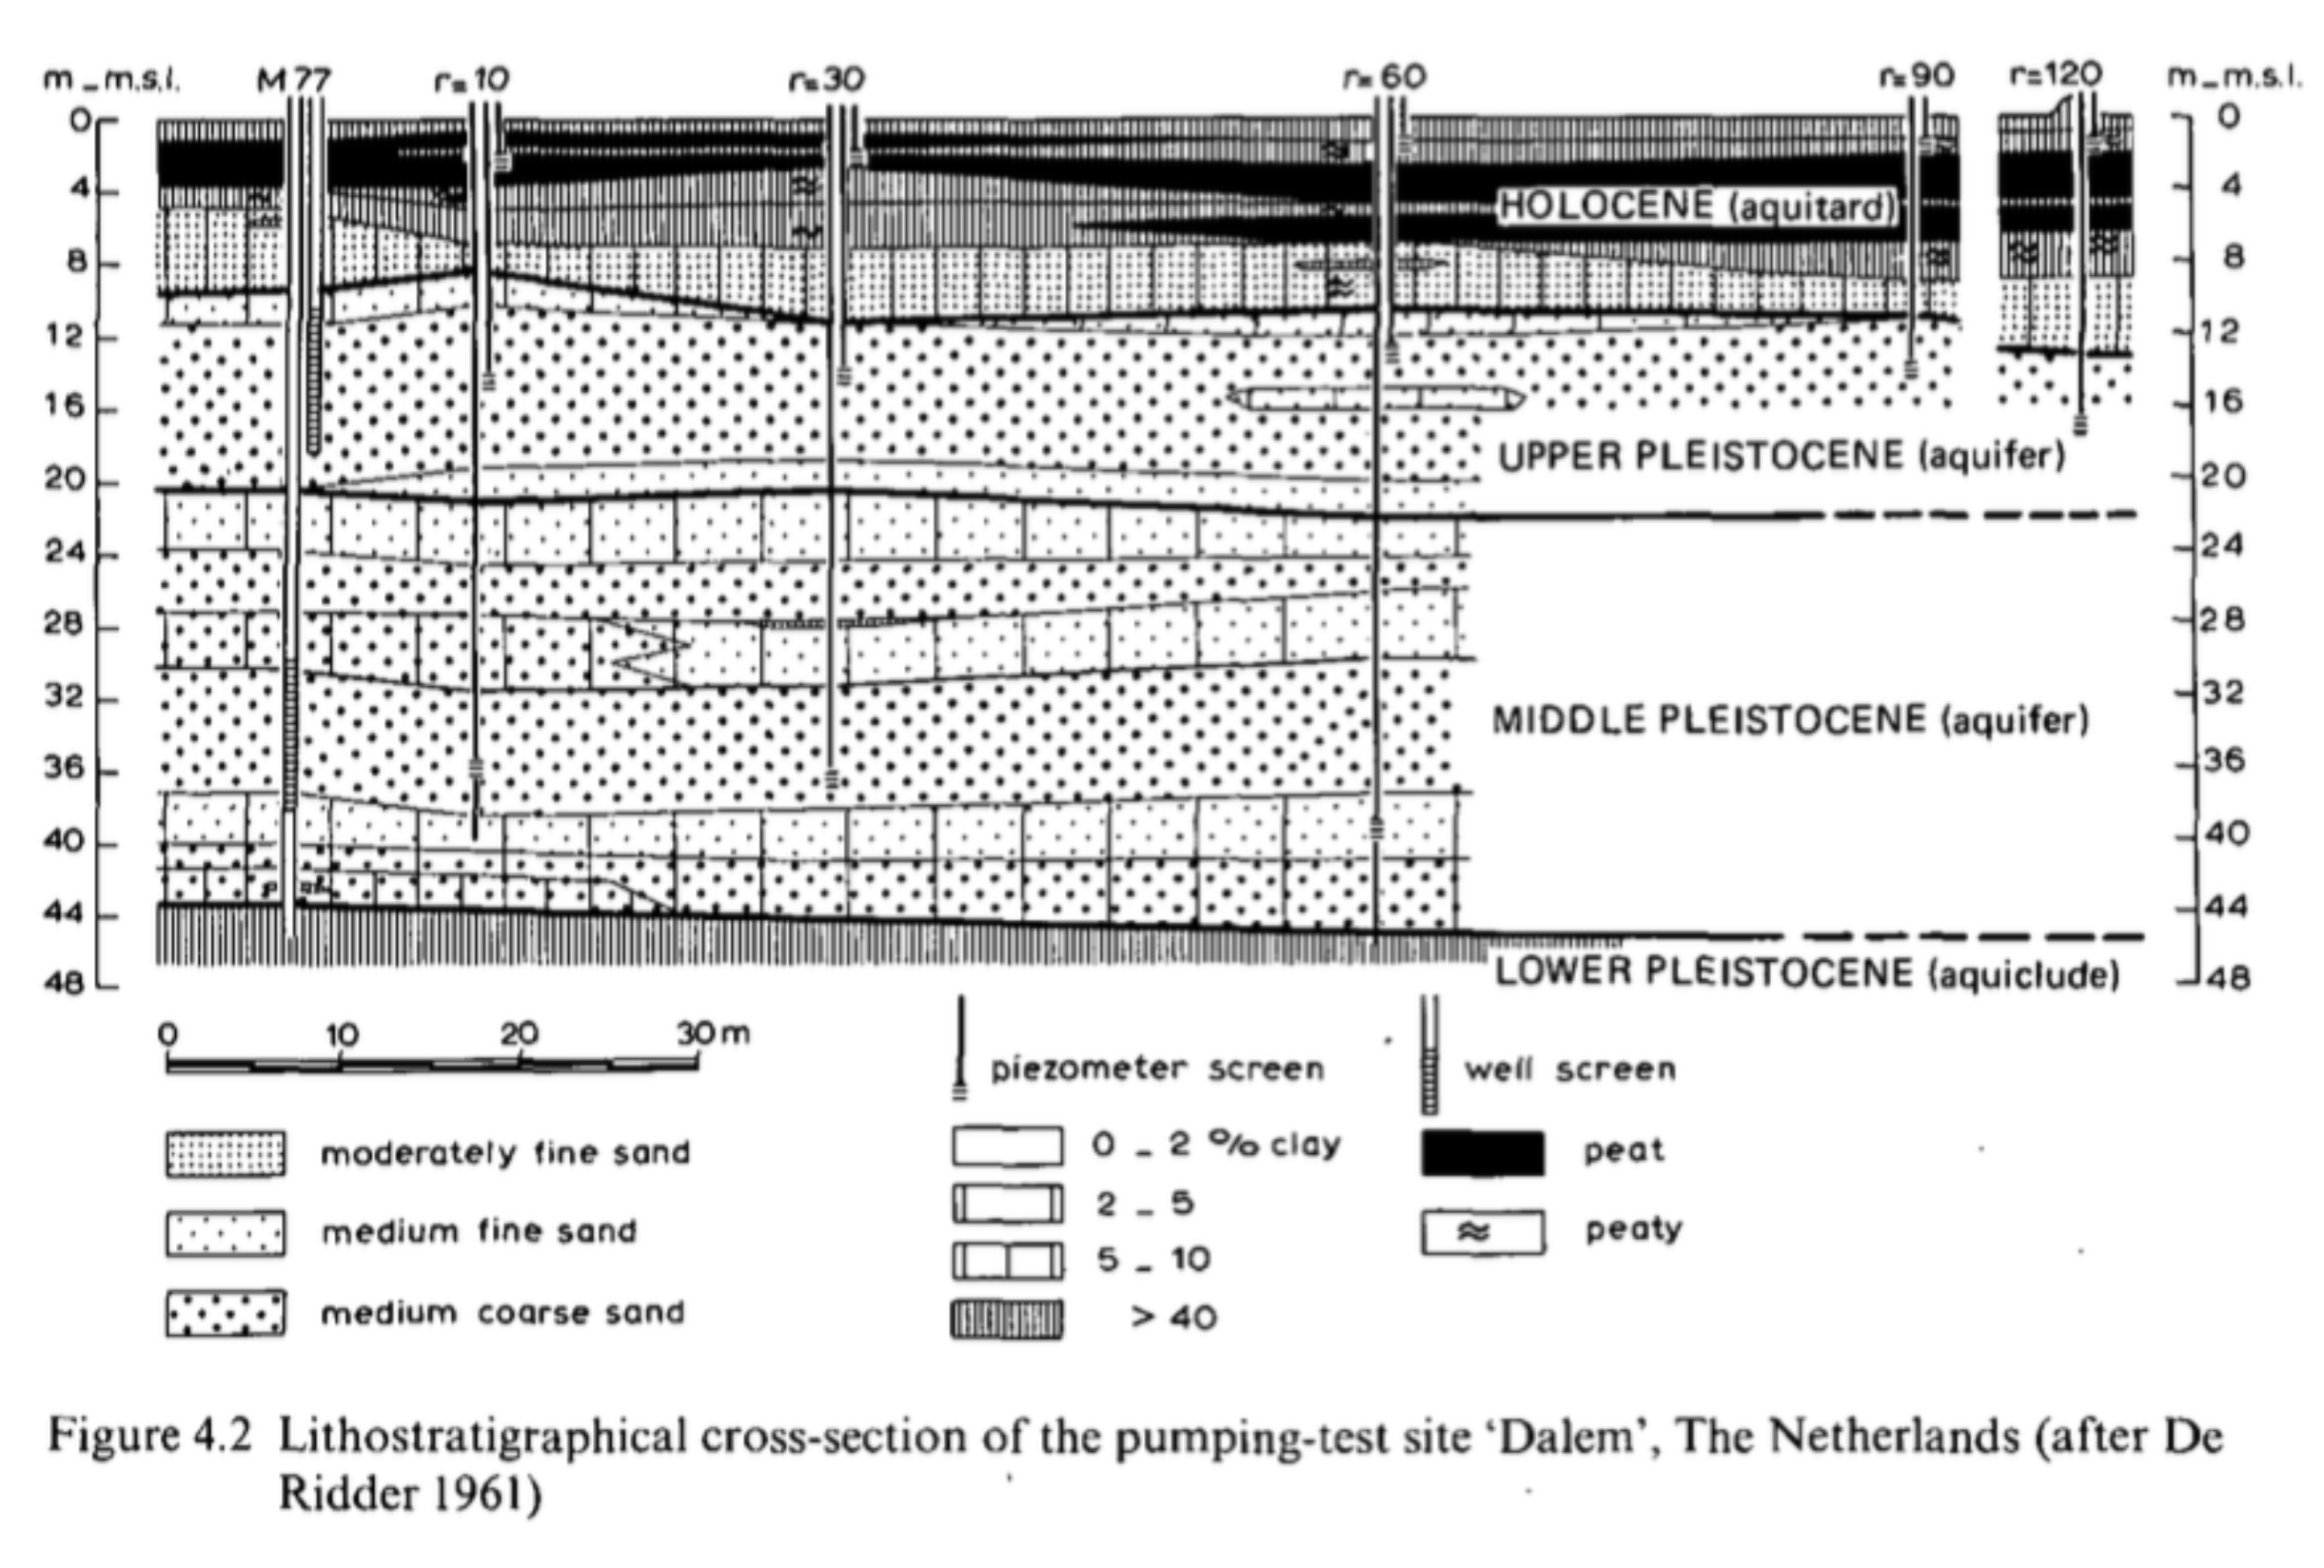
\includegraphics[width=0.8\textwidth]{pictures/Dalem_cross_sectioin}

\caption{Cross section pumping test Dalem (Kruseman \& De Ridder, 1970, 1994)}

\end{figure}

The data are given below in a csv form:

\inputencoding{latin9}\begin{lstlisting}
t(min),s_piez1,s_piez2,s_piez3,t/(r1)^2,t/(r2)^2,t/(r3)^2,u,1/u,w(u)
,m,m,m,,,,,,
1,0.2,0.07,0,0.043252595,0.000307865,7.24049E-05,0.001,1000,6.33
2,0.25,0.08,0.03,0.08650519,0.000615729,0.00014481,0.001584893,630.9573445,5.87
3,0.24,0.1,0.03,0.129757785,0.000923594,0.000217215,0.002511886,398.1071706,5.41
4,0.27,0.1,0.05,0.173010381,0.001231459,0.00028962,0.003981072,251.1886432,4.95
5,0.27,0.11,0.05,0.216262976,0.001539324,0.000362024,0.006309573,158.4893192,4.49
6,0.26,0.1,0.06,0.259515571,0.001847188,0.000434429,0.01,100,4.04
7,0.27,0.11,0.05,0.302768166,0.002155053,0.000506834,0.015848932,63.09573445,3.58
8,0.28,0.12,0.06,0.346020761,0.002462918,0.000579239,0.025118864,39.81071706,3.13
9,0.29,0.13,0.06,0.389273356,0.002770782,0.000651644,0.039810717,25.11886432,2.69
10,0.28,0.14,0.07,0.432525952,0.003078647,0.000724049,0.063095734,15.84893192,2.25
11,0.3,0.13,0.08,0.475778547,0.003386512,0.000796454,0.1,10,1.82
12,0.27,0.14,0.07,0.519031142,0.003694377,0.000868859,0.158489319,6.309573445,1.42
13,0.3,0.13,0.08,0.562283737,0.004002241,0.000941264,0.251188643,3.981071706,1.04
14,0.28,0.11,0.09,0.605536332,0.004310106,0.001013669,0.398107171,2.511886432,0.71
15,0.3,0.12,0.08,0.648788927,0.004617971,0.001086073,0.630957344,1.584893192,0.43
20,0.3,0.14,0.09,0.865051903,0.006157294,0.001448098,1,1,0.22
25,0.3,0.13,0.09,1.081314879,0.007696618,0.001810122,1.584893192,0.630957344,0.09
30,0.32,0.15,0.1,1.297577855,0.009235941,0.002172147,2.511886432,0.398107171,0.02
35,0.31,0.17,0.11,1.51384083,0.010775265,0.002534171,3.981071706,0.251188643,0.00
40,0.32,0.13,0.1,1.730103806,0.012314588,0.002896196,6.309573445,0.158489319,0.00
45,0.33,0.16,0.13,1.946366782,0.013853912,0.00325822,10,0.1,0.00
50,0.32,0.18,0.14,2.162629758,0.015393236,0.003620245,15.84893192,0.063095734,0.00
55,0.35,0.18,0.11,2.378892734,0.016932559,0.003982269,25.11886432,0.039810717,0.00
60,0.34,0.17,0.13,2.595155709,0.018471883,0.004344294,39.81071706,0.025118864,0.00
75,0.34,0.17,0.14,3.243944637,0.023089853,0.005430367,63.09573445,0.015848932,0.00
90,0.35,0.18,0.14,3.892733564,0.027707824,0.006516441,100,0.01,0.00
105,0.35,0.18,0.14,4.541522491,0.032325795,0.007602514,,,
120,0.36,0.2,0.14,5.190311419,0.036943765,0.008688588,,,
135,0.35,0.19,0.13,5.839100346,0.041561736,0.009774661,,,
150,0.36,0.19,0.13,6.487889273,0.046179707,0.010860735,,,
165,0.35,0.19,0.15,7.136678201,0.050797677,0.011946808,,,
180,0.4,0.21,0.16,7.785467128,0.055415648,0.013032882,,,
195,0.36,0.2,0.16,8.434256055,0.060033619,0.014118955,,,
210,0.36,0.2,0.14,9.083044983,0.06465159,0.015205029,,,
225,0.36,0.21,0.15,9.73183391,0.06926956,0.016291102,,,
240,0.38,0.21,0.16,10.38062284,0.073887531,0.017377176,,,
270,0.39,0.22,0.15,11.67820069,0.083123472,0.019549323,,,
300,0.38,0.21,0.16,12.97577855,0.092359414,0.02172147,,,
330,0.36,0.22,0.16,14.2733564,0.101595355,0.023893617,,,
360,0.37,0.2,0.17,15.57093426,0.110831296,0.026065764,,,
390,0.39,0.21,0.16,16.86851211,0.120067238,0.028237911,,,
420,0.4,0.23,0.2,18.16608997,0.129303179,0.030410058,,,
450,0.38,0.23,0.17,19.46366782,0.13853912,0.032582205,,,
480,0.39,0.22,0.18,20.76124567,0.147775062,0.034754352,,,
510,0.38,0.22,0.17,22.05882353,0.157011003,0.036926499,,,
540,0.39,0.23,0.17,23.35640138,0.166246944,0.039098646,,,
570,0.39,0.2,0.18,24.65397924,0.175482886,0.041270793,,,
600,0.38,0.24,0.17,25.95155709,0.184718827,0.04344294,,,
1320,0.39,0.23,0.16,57.09342561,0.40638142,0.095574468,,,
1380,0.4,0.23,0.19,59.68858131,0.424853302,0.099918762,,,
1440,0.39,0.23,0.17,62.28373702,0.443325185,0.104263056,,,
1500,0.42,0.21,0.18,64.87889273,0.461797068,0.10860735,,,
1560,0.4,0.23,0.16,67.47404844,0.480268951,0.112951644,,,
1620,0.4,0.24,0.19,70.06920415,0.498740833,0.117295938,,,
1680,0.38,0.22,0.2,72.66435986,0.517212716,0.121640232,,,
1740,0.4,0.23,0.17,75.25951557,0.535684599,0.125984526,,,
1800,0.4,0.25,0.2,77.85467128,0.554156481,0.13032882,,,
1860,0.4,0.24,0.18,80.44982699,0.572628364,0.134673114,,,
1920,0.4,0.25,0.19,83.0449827,0.591100247,0.139017408,,,
2880,0.41,0.25,0.2,124.567474,0.88665037,0.208526111,,,
3360,0.39,0.23,0.19,145.3287197,1.034425432,0.243280463,,,
4320,0.4,0.23,0.18,186.8512111,1.329975556,0.312789167,,,
4800,0.4,0.23,0.2,207.6124567,1.477750617,0.347543519,,,
5760,0.38,0.23,0.18,249.1349481,1.773300741,0.417052223,,,
6240,0.38,0.24,0.17,269.8961938,1.921075802,0.451806575,,,
7200,0.39,0.23,0.18,311.4186851,2.216625926,0.521315278,,,
7680,0.38,0.23,0.2,332.1799308,2.364400988,0.55606963,,,
8640,0.39,0.22,0.17,373.7024221,2.659951111,0.625578334,,,
9120,0.39,0.23,0.18,394.4636678,2.807726173,0.660332686,,,
10080,0.4,0.23,0.19,435.9861592,3.103276296,0.72984139,,,
10560,0.41,0.24,0.17,456.7474048,3.251051358,0.764595742,,,
11520,0.4,0.24,0.19,498.2698962,3.546601481,0.834104446,,,
12000,0.41,0.24,0.19,519.0311419,3.694376543,0.868858797,,,
12960,0.41,0.25,0.19,560.5536332,3.989926667,0.938367501,,,
13440,0.39,0.23,0.17,581.3148789,4.137701728,0.973121853,,,
14400,0.39,0.22,0.19,622.8373702,4.433251852,1.042630557,,,
14880,0.4,0.23,0.16,643.5986159,4.581026914,1.077384909,,,
15840,0.39,0.24,0.19,685.1211073,4.876577037,1.146893613,,,
16320,0.39,0.23,0.17,705.8823529,5.024352099,1.181647964,,,
17280,0.41,0.25,0.19,747.4048443,5.319902222,1.251156668,,,
17760,0.4,0.22,0.19,768.16609,5.467677284,1.28591102,,,
18720,0.39,0.22,0.18,809.6885813,5.763227407,1.355419724,,,
19200,0.39,0.24,0.18,830.449827,5.911002469,1.390174076,,,
20160,0.38,0.24,0.19,871.9723183,6.206552593,1.45968278,,,
20640,0.39,0.24,0.18,892.733564,6.354327654,1.494437132,,,
21600,0.39,0.23,0.16,934.2560554,6.649877778,1.563945835,,,
22080,0.41,0.22,0.18,955.017301,6.797652839,1.598700187,,,
23040,0.4,0.22,0.17,996.5397924,7.093202963,1.668208891,,,
23520,0.4,0.23,0.18,1017.301038,7.240978025,1.702963243,,,
24480,0.41,0.25,0.2,1058.823529,7.536528148,1.772471947,,,
24960,0.4,0.23,0.19,1079.584775,7.68430321,1.807226299,,,
25920,0.4,0.24,0.18,1121.107266,7.979853333,1.876735002,,,
26400,0.38,0.23,0.18,1141.868512,8.127628395,1.911489354,,,
27360,0.4,0.23,0.18,1183.391003,8.423178518,1.980998058,,,
27840,0.38,0.24,0.19,1204.152249,8.57095358,2.01575241,,,
28800,0.39,0.25,0.18,1245.67474,8.866503704,2.085261114,,,
29280,0.4,0.23,0.19,1266.435986,9.014278765,2.120015466,,,
30240,0.4,0.24,0.18,1307.958478,9.309828889,2.189524169,,,
30720,0.41,0.23,0.17,1328.719723,9.457603951,2.224278521,,,
31680,0.4,0.23,0.19,1370.242215,9.753154074,2.293787225,,,
32160,0.41,0.24,0.19,1391.00346,9.900929136,2.328541577,,,
33120,0.4,0.24,0.19,1432.525952,10.19647926,2.398050281,,,
33600,0.39,0.23,0.18,1453.287197,10.34425432,2.432804633,,,
34560,0.4,0.22,0.17,1494.809689,10.63980444,2.502313337,,,
35040,0.4,0.23,0.2,1515.570934,10.78757951,2.537067688,,,
36000,0.41,0.22,0.19,1557.093426,11.08312963,2.606576392,,,
36480,0.39,0.24,0.18,1577.854671,11.23090469,2.641330744,,,
37440,0.4,0.23,0.18,1619.377163,11.52645481,2.710839448,,,
37920,0.41,0.24,0.21,1640.138408,11.67422988,2.7455938,,,
38880,0.4,0.22,0.2,1681.6609,11.96978,2.815102504,,,
39360,0.4,0.22,0.17,1702.422145,12.11755506,2.849856856,,,
40320,0.42,0.23,0.17,1743.944637,12.41310519,2.919365559,,,
40800,0.38,0.22,0.19,1764.705882,12.56088025,2.954119911,,,
41760,0.4,0.23,0.18,1806.228374,12.85643037,3.023628615,,,
42240,0.4,0.24,0.19,1826.989619,13.00420543,3.058382967,,,
43200,0.38,0.22,0.17,1868.512111,13.29975556,3.127891671,,,
43680,0.38,0.24,0.19,1889.273356,13.44753062,3.162646023,,,
44640,0.4,0.24,0.19,1930.795848,13.74308074,3.232154726,,,
45120,0.4,0.23,0.19,1951.557093,13.8908558,3.266909078,,,
46080,0.4,0.24,0.17,1993.079585,14.18640593,3.336417782,,,
46560,0.39,0.24,0.18,2013.84083,14.33418099,3.371172134,,,
47520,0.41,0.23,0.19,2055.363322,14.62973111,3.440680838,,,
48000,0.38,0.24,0.19,2076.124567,14.77750617,3.47543519,,,
48960,0.4,0.23,0.17,2117.647059,15.0730563,3.544943893,,,
49440,0.39,0.22,0.19,2138.408304,15.22083136,3.579698245,,,
50400,0.38,0.23,0.16,2179.930796,15.51638148,3.649206949,,,
50880,0.41,0.24,0.19,2200.692042,15.66415654,3.683961301,,,
51840,0.41,0.22,0.18,2242.214533,15.95970667,3.753470005,,,
52320,0.39,0.23,0.21,2262.975779,16.10748173,3.788224357,,,
53280,0.4,0.25,0.2,2304.49827,16.40303185,3.857733061,,,
53760,0.4,0.25,0.19,2325.259516,16.55080691,3.892487412,,,
54720,0.41,0.24,0.19,2366.782007,16.84635704,3.961996116,,,
55200,0.39,0.24,0.18,2387.543253,16.9941321,3.996750468,,,
56160,0.4,0.25,0.19,2429.065744,17.28968222,4.066259172,,,
56640,0.39,0.22,0.17,2449.82699,17.43745728,4.101013524,,,
57600,0.38,0.23,0.17,2491.349481,17.73300741,4.170522228,,,
58080,0.39,0.23,0.17,2512.110727,17.88078247,4.205276579,,,
59040,0.39,0.23,0.19,2553.633218,18.17633259,4.274785283,,,
59520,0.39,0.25,0.18,2574.394464,18.32410765,4.309539635,,,
60480,0.39,0.23,0.19,2615.916955,18.61965778,4.379048339,,,
60960,0.4,0.22,0.18,2636.678201,18.76743284,4.413802691,,,
61920,0.41,0.24,0.18,2678.200692,19.06298296,4.483311395,,,
62400,0.39,0.23,0.19,2698.961938,19.21075802,4.518065747,,,
63360,0.39,0.22,0.19,2740.484429,19.50630815,4.58757445,,,
63840,0.39,0.23,0.17,2761.245675,19.65408321,4.622328802,,,
64800,0.42,0.24,0.18,2802.768166,19.94963333,4.691837506,,,
65280,0.39,0.24,0.19,2823.529412,20.09740839,4.726591858,,,
66240,0.39,0.25,0.17,2865.051903,20.39295852,4.796100562,,,
66720,0.39,0.24,0.19,2885.813149,20.54073358,4.830854914,,,
67680,0.39,0.23,0.19,2927.33564,20.8362837,4.900363617,,,
68160,0.4,0.21,0.2,2948.096886,20.98405877,4.935117969,,,
69120,0.39,0.24,0.2,2989.619377,21.27960889,5.004626673,,,
69600,0.38,0.25,0.17,3010.380623,21.42738395,5.039381025,,,
70560,0.39,0.23,0.17,3051.903114,21.72293407,5.108889729,,,
71040,0.4,0.23,0.18,3072.66436,21.87070914,5.143644081,,,
72000,0.39,0.24,0.16,3114.186851,22.16625926,5.213152784,,,
72480,0.4,0.25,0.16,3134.948097,22.31403432,5.247907136,,,
73440,0.38,0.24,0.19,3176.470588,22.60958444,5.31741584,,,
73920,0.41,0.25,0.18,3197.231834,22.75735951,5.352170192,,,
74880,0.41,0.23,0.19,3238.754325,23.05290963,5.421678896,,,
75360,0.39,0.22,0.18,3259.515571,23.20068469,5.456433248,,,
76320,0.4,0.23,0.18,3301.038062,23.49623481,5.525941952,,,
76800,0.41,0.24,0.19,3321.799308,23.64400988,5.560696303,,,
77760,0.38,0.22,0.2,3363.321799,23.93956,5.630205007,,,
78240,0.4,0.24,0.19,3384.083045,24.08733506,5.664959359,,,
79200,0.38,0.23,0.18,3425.605536,24.38288518,5.734468063,,,
79680,0.4,0.23,0.18,3446.366782,24.53066025,5.769222415,,,
80640,0.39,0.24,0.18,3487.889273,24.82621037,5.838731119,,,
81120,0.39,0.24,0.18,3508.650519,24.97398543,5.873485471,,,
82080,0.41,0.22,0.18,3550.17301,25.26953556,5.942994174,,,
82560,0.39,0.23,0.18,3570.934256,25.41731062,5.977748526,,,
83520,0.41,0.23,0.18,3612.456747,25.71286074,6.04725723,,,
84000,0.38,0.23,0.17,3633.217993,25.8606358,6.082011582,,,
84960,0.41,0.25,0.19,3674.740484,26.15618593,6.151520286,,,
85440,0.42,0.23,0.19,3695.50173,26.30396099,6.186274638,,,
86400,0.41,0.24,0.18,3737.024221,26.59951111,6.255783341,,,
86880,0.41,0.24,0.18,3757.785467,26.74728617,6.290537693,,,
\end{lstlisting}
\inputencoding{utf8}
\end{document}
